\documentclass[a4paper,12pt]{article}
\usepackage[utf8]{inputenc}
\usepackage[cm,empty]{fullpage}
\usepackage[T2A]{fontenc}
\usepackage[english, russian]{babel}
\usepackage{amssymb,amsmath,amsxtra,amsthm}
\usepackage{proof}
\usepackage[pdftex]{graphicx}
\usepackage{wrapfig}
\usepackage{skak}
\usepackage{xcolor}
\usepackage{braket}

\usepackage[left=2cm,right=2cm,
    top=1cm,bottom=1cm,bindingoffset=0cm]{geometry}

\renewcommand{\leq}{\leqslant}
\renewcommand{\geq}{\geqslant}


\newcommand{\iiff}{\Longleftrightarrow}
\renewcommand{\iff}{\Leftrightarrow}
\newcommand{\nothing}{\varnothing}


\newcommand{\NN}{\mathbb{N}}
\newcommand{\ZZ}{\mathbb{Z}}
\newcommand{\Q}{\mathbb{Q}}
\newcommand{\A}{\mathbb{A}}
\newcommand{\R}{\mathbb{R}}
\renewcommand{\C}{\mathbb{C}}

\renewcommand{\phi}{\varphi}
\newcommand{\eps}{\varepsilon}

\newcounter{z}


\newcommand{\zs}{\refstepcounter{z}\vskip 10pt\par\noindent
\fbox{\textbf{12.\arabic{z}}} }

\newcommand{\z}{\refstepcounter{z}\vskip 20pt\noindent
\fbox{\textbf{\arabic{z}}} }

\renewcommand{\date}{{\bf 31 января 2021}} 

\newcommand{\dif}
{
------------------------------------------------------------------------------------------------------------------------------------------------------
}

\newcommand{\HSEhat}{
\vspace*{-0pt}
\noindent
\setcounter{z}{0}
\vspace*{-10pt}

\vspace{-20pt}


{\bf \phantom{\date}  \large \hfill Дискретная математика: \hfill \normalsize \date}

\vspace{5 pt}
{\bf \large \hfill  неориентированные графы.\hfill }

\vspace{15 pt}
\centerline{ \large  Домашнее задание №3.}

\vspace{15 pt}
\centerline{ \large  Кирилл Сетдеков}


\vspace*{10pt}
\setcounter{z}{0}

}

\begin{document}

\HSEhat

Всюду ниже рассматриваются только графы {\bf без петель} и {\bf кратных ребер}.


\begin{center}
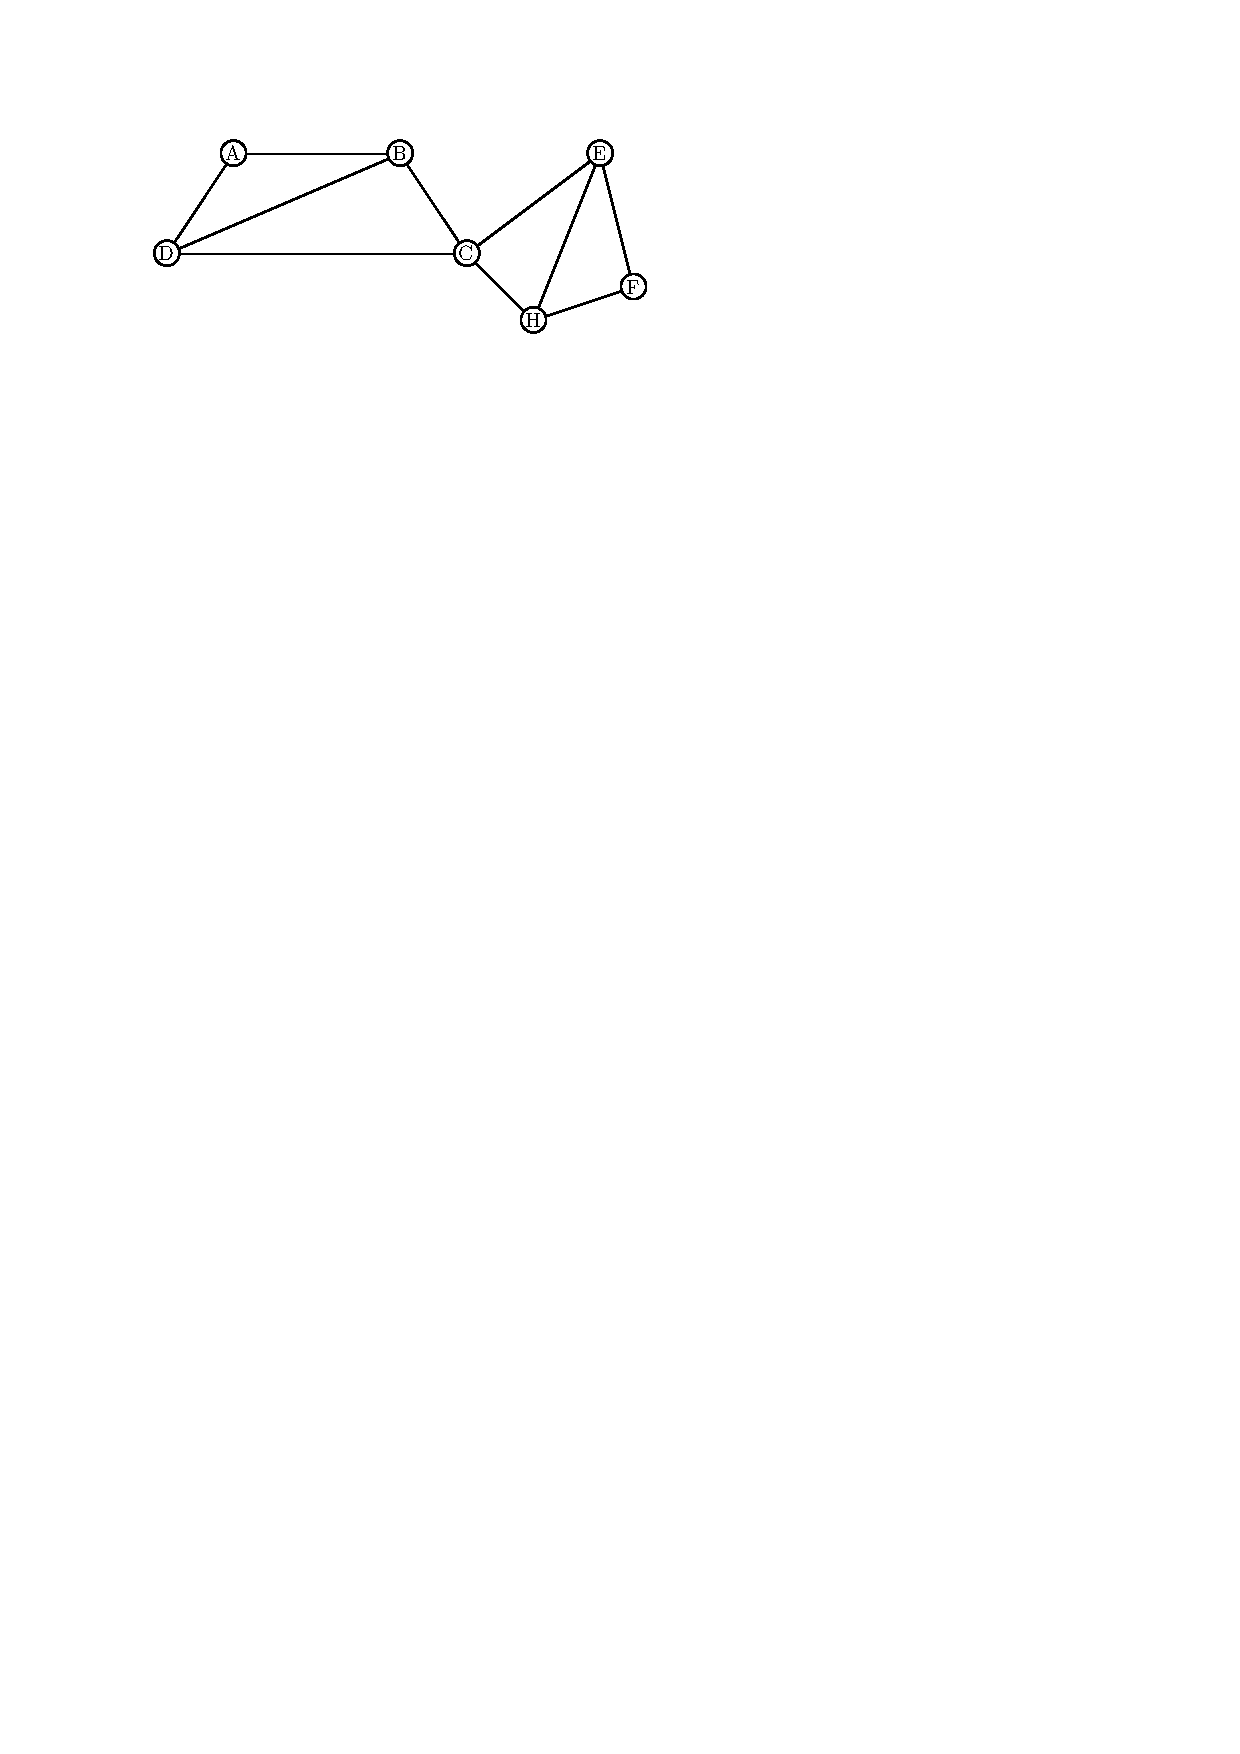
\includegraphics[scale=1]{img/graphHW.pdf}
\end{center}
\vspace{-15 pt}

\z Граф $G$ изображен на рисунке выше.

{\bf а)} Найдите максимальную длину простого цикла в графе $G$. Укажите
все различные простые циклы максимальной длины.

\textbf{Ответ: Максимальная длина простого цикла = 4. Цикл из вершин $(A,B,C,D, A)$ и $(C,E,F,H, C)$. Каждому циклу соответствует 8 путей (начинающиеся в каждой из 4 вершин по часовой стрелке и против часовой стрелки), всего 16 путей}

{\bf б)} Верно ли, что если в графе $G$ удалить любое ребро, то из любой его
вершины можно будет добраться до любой? При положительном ответе
приведите обоснование, при отрицательном --- укажите ребро, которое
можно удалить, и вершины, между которыми не будет пути.

\textbf{Решение:} \\
Заметим, что в этом графе есть 4 цикла длиной 3 состоящие из 3 вершин: \\ $(A,B,D, A), (B,C,D, B), (C,E,H, C), (E,F,H, E)$. Каждое из ребер графа принадлежит к одному из этих циклов. Исходный граф $G$ - имеет одну компоненту связности и можно найти путь между любой парой вершин.

Предположим, что мы удалили случайное ребро. Это ребро принадлежало одному из циклов, указанных выше.
Рассмотрим все пары вершин $\set{v, u}$. Так как мы могли построить путь от каждой вершины к каждой, $\forall v,u \in G, v \sim u$
Для каждого возможного пути после удаления случайного ребра верно или:

1) Путь от $v$ к $u$ не содержал удаленное ребро. Следовательно эта пара вершин достижима друг от друга $v \sim u$

2) Путь от $v$ к $u$ содержал удаленное ребро $\set{r_1, r_2}$. Тогда для цикла, который содержал вершины $r_1, r_2$ пройдем в другую сторону по циклю и построим путь от $r_1$ до $r_2$. Заменим таким образом часть удаленного пути. Следовательно эта пара вершин также достижима друг от друга $v \sim u$

Мы получили из 1) и 2) что $\forall v,u \in G, v \sim u$, что означает что граф остался связным.

\textbf{Ответ: Да}

{\bf в)} Какое минимальное количество рёбер необходимо удалить из графа $G$, чтобы он стал несвязным?

\textbf{Решение:} \\
В прошлом пункте мы показали, что для 1 ребра - граф останется связным. Для случая 2 ребра можно привести пример: удалим ребро $\set{B, C}$ и $\set{D, C}$. В графе останется 2 компоненты связности.

\textbf{Ответ: 2 ребра}

\z В государстве $100$ городов, и из каждого из них выходит $4$ дороги в другие города этого государства. Сколько всего дорог в государстве?

\textbf{Решение:} \\
Предположим, что мы нарисовали граф дорог, где каждый город - вершина, а дорога - ребро. Число вершин $|V| = 100$, а степень каждой вершины = 4.
Следовательно сумма степеней всех вершин:
$$\sum_{v_i \in V}{deg(v_i)} = 4\times100 = 400 = 2|E|$$
где $|E|$ - число ребер.
$$400 = 2|E|$$
$$|E| = 200$$
Так как дороги - ребра, то число дорог равно числу ребер.

\textbf{Ответ: 200 дорог}
\z Можно ли нарисовать картинки на рисунке ниже, не отрывая карандаша от бумаги и проходя по каждой линии по одному разу?

Если можно, то покажите, как это сделать.

Если нельзя, то докажите, что это сделать невозможно.
\vspace{-40 pt}
\begin{center}
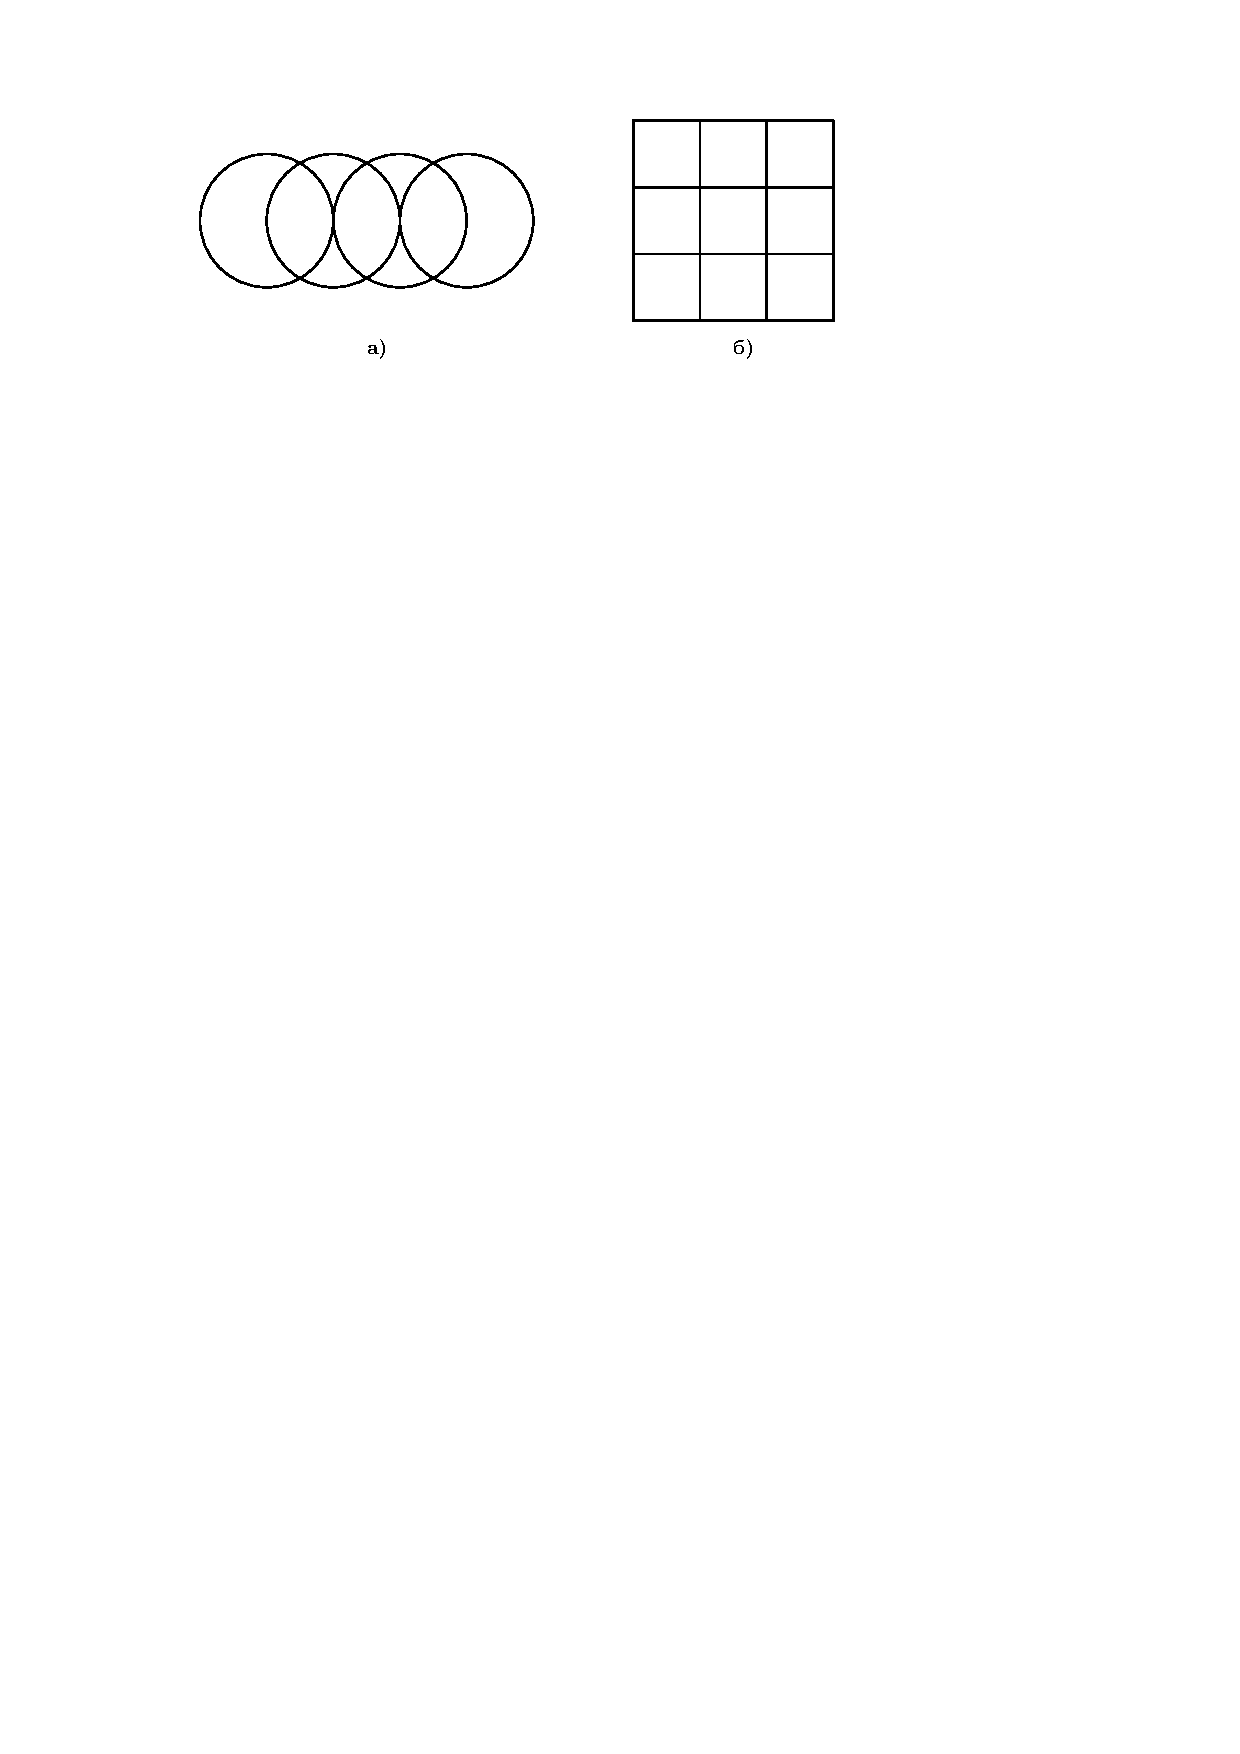
\includegraphics[scale=1]{img/graphHW2.pdf}
\end{center}
\vspace{-15 pt}

{\bf а)} 
\textbf{Решение:} \\
Начнем с точки S. Обозначим каждую кривую между точками пересечения числом. Из точки S обведем фигуру по периметру, проходя по кривым в таком порядке $1 \to 2 \to 3 \to 4 \to 5 \to 6$. После этого проведем линию по кривым $7 \to 8 \to 9 \to 10 \to 11 \to 12$. Далее вернемся в точку S пройдя по кривым $13 \to 14 \to 15 \to 16$


\begin{center}
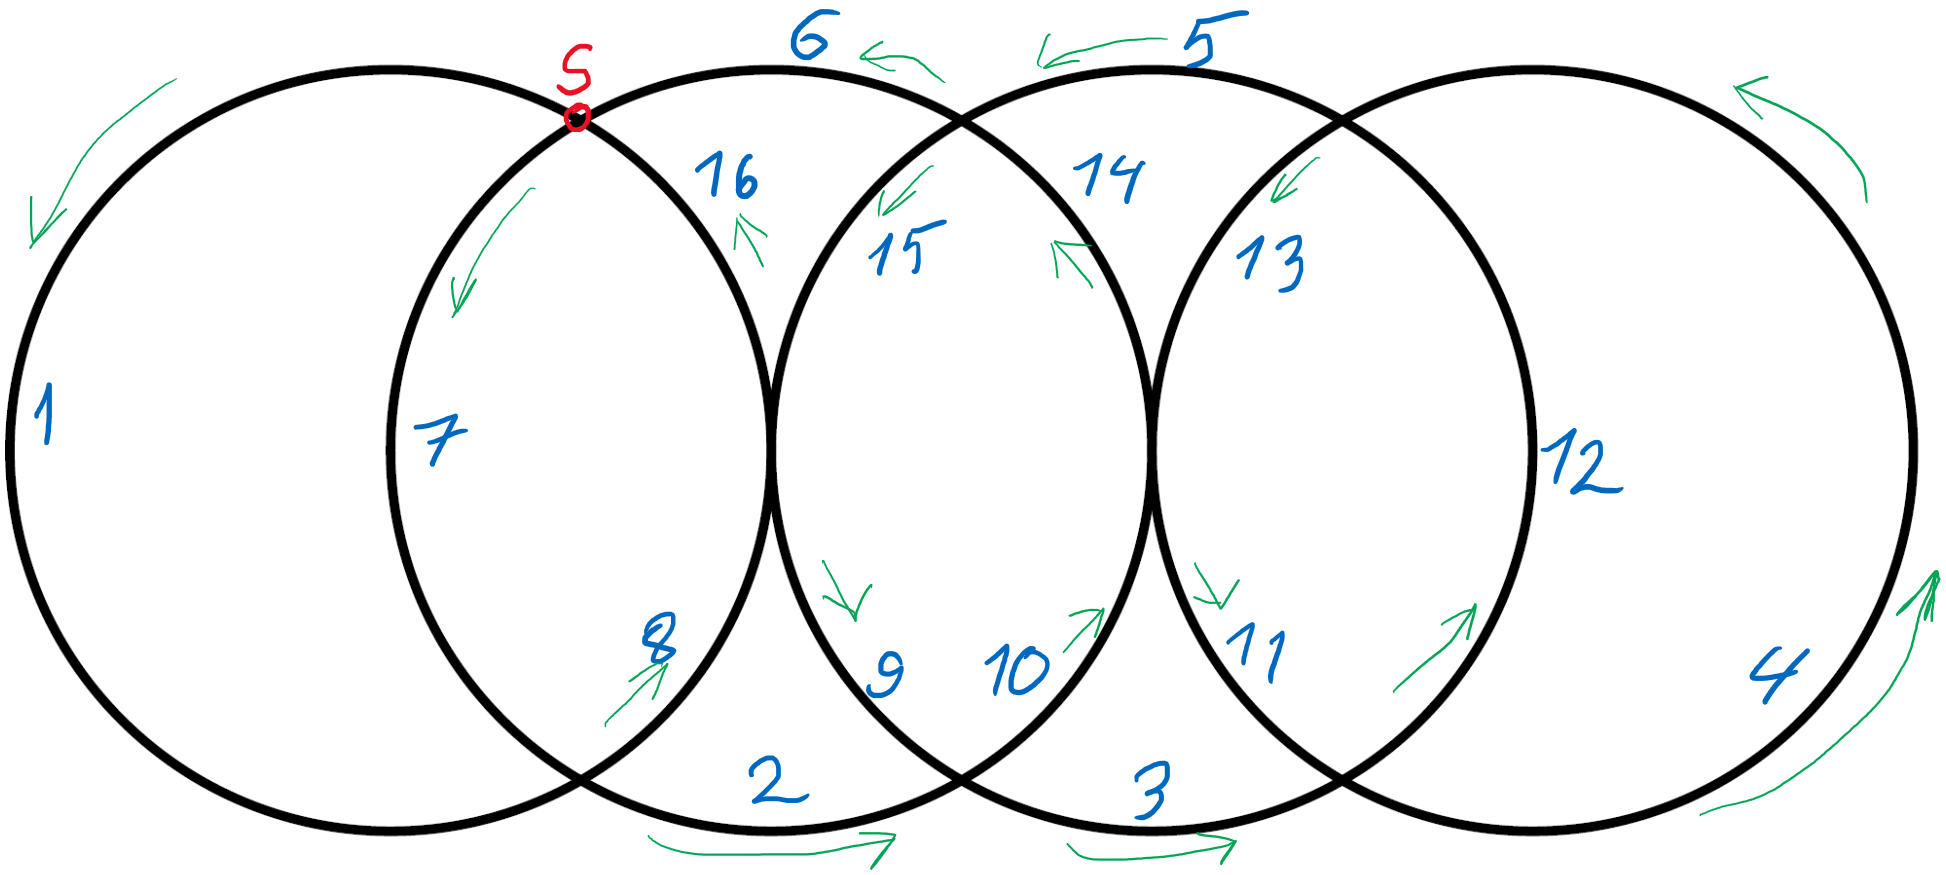
\includegraphics[width=\textwidth]{img/path.png}
\end{center}


\textbf{Ответ: Можно, решение приведено на рисунке выше.}

{\bf б)} 
\textbf{Решение:} \\
Воспользуемся теоремой о существовании эйлерова цикла.

В графе G = (V,E) существует эйлеров цикл $\Leftrightarrow$ все вершины имеют четную степень.

Если эйлеров цикл не существует $\Rightarrow$ нельзя построить путь, который пройдет по каждому ребру 1 раз и вернется в исходную вершину $\Rightarrow$ нельзя нарисовать картинки на рисунке ниже, не отрывая карандаша от бумаги и проходя по каждой линии по одному разу

Представим что на картинке изображен граф, где 16 вершин, находящихся на пересечении вертикальных и горизонтальных линий.

Запишем их степени в матрицу, где положение числа соответствует положению вершины:

$$\begin{pmatrix}
2 & 3 & 3 & 2\\
3 & 4 & 4 & 3\\
3 & 4 & 4 & 3\\
2 & 3 & 3 & 2
\end{pmatrix}$$

Среди вершин есть такие, где $deg(v) =3$ $\Rightarrow$ в графе, который мы представили не существует эйлеров цикл $\Rightarrow$ нельзя нарисовать картинки на рисунке ниже, не отрывая карандаша от бумаги и проходя по каждой линии по одному разу

\textbf{Ответ: Нельзя}

\z В дереве на $2020$ вершинах ровно три вершины имеют степень $1$.
Сколько вершин имеют степень $3$?

\textbf{Решение:} \\
В нашем дереве $|V| = 2020$. Так как это дерево, в нем $|E| = |V|-1 =2019$ ребер. Сумма степеней вершин для графа $$\sum_{v_i \in V}{deg(v_i)} = 2|E| = 4038$$
Согласно условию - $N(deg(v_i) =1)=3$ число вершин со степенью 1. 
Для дерева с 3 листьями, максимальная степень вершин меньше или равна 3.

Начнем решать задачу, предположив, что в дереве есть вершины со степенью 1, 2 и 3.

Обозначим как x и y число вершин со степенью 3 и 2.
$$N(deg(v_i) =3)=x; N(deg(v_i) =2)=y$$.
Составим систему уравнений.
$$\begin{cases} 3+2y + 3x = 4038 \\ x+y+3 = 2020\end{cases} \Rightarrow \begin{cases} 2y + 3x = 4035 \\ y = 2017-x\end{cases}\Rightarrow  \begin{cases} 2(2017-x) + 3x = 4035 \\ y = 2017-x\end{cases}\Rightarrow $$
$$
\Rightarrow  \begin{cases} 4034-2x + 3x = 4035 \\ y = 2017-x\end{cases}\Rightarrow  \begin{cases} x = 1 \\ y = 2016\end{cases}
$$

Мы получили 1 вершину со степенью 3 и 2016 вершин со степенью 2.

Предположим, что есть вершины со степенью 

\textbf{Ответ: Одна вершина}

\z У некоторого графа на $6$ вершинах ровно $11$ ребер. Докажите, что этот граф связен.

\textbf{Решение:} \\
Известно, что для графа с $n$ вершинами, максимально число ребер для несвязного графа = $\frac{(n-1)(n-2)}{2}$. Для нашего графа $n=|V| = 6$:
$$\frac{(n-1)(n-2)}{2}=\frac{5\times4}{2}=10$$

Такой несвязный граф будет состоять из двух компонент связности, в одной 1 вершина и 0 ребер, во второй - 5 вершин и 10 ребер. Во второй половине графа - компонента связности является полной так как в ней все вершины соединены между собой.

Предположим, что мы взяли несвязный граф с 10 ребрами и 6 вершинами, описанный в абзаце выше и смогли добавить еще одно ребро и получить граф, который не связен. Возможно 1 из трех вариантов:

1) Мы добавили ребро между компонентами связности - мы получили граф с одной компонентой связности - противоречие с предположением

2) Мы добавили ребро в компоненту связности из 1 вершины - так как мы рассматриваем граф без петель - мы не смогли добавить в эту компоненту ребро - противоречие с предположением

3) Мы добавили ребро в компоненту связности из 5 вершины - эта компонента связности уже полный граф - мы не смогли добавить в эту компоненту ребро - противоречие с предположением

Следовательно предположение "мы взяли несвязный граф с 10 ребрами и 6 вершинами и смогли добавить еще одно ребро и получить граф, который не связен" не верно $\Rightarrow$ граф из 6 вершин и 10 ребер - связан

\textbf{Ответ: Граф связан}

\z Можно ли за несколько ходов (по шахматным правилам и не выходя за пределы доски $3\times 3$) поставить коней так, чтобы из расположения на левой картинке получилось расположение коней на правой?

Если можно, то укажите последовательность шагов.

Если нельзя, то докажите, что это сделать невозможно.

\begin{center}
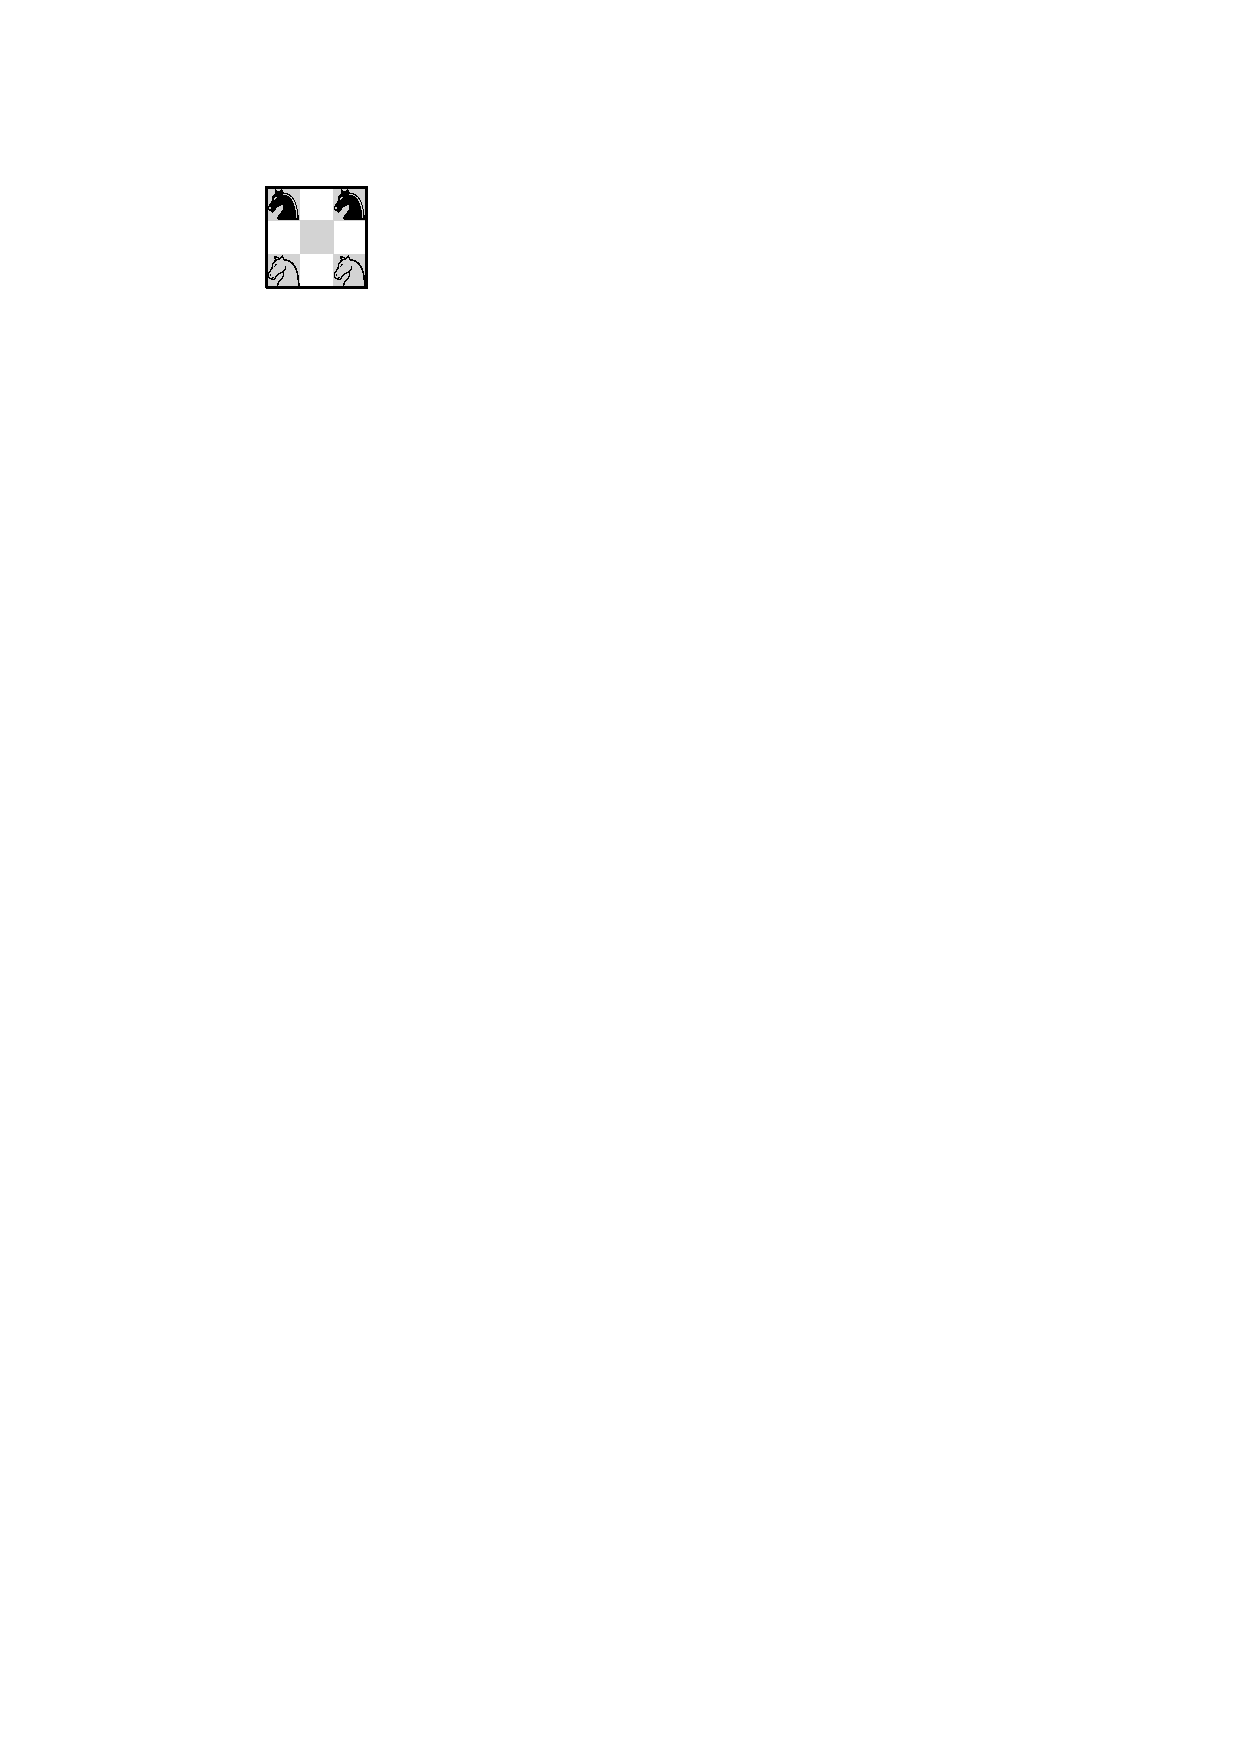
\includegraphics[scale=1.5]{img/Knights1.pdf}\qquad \qquad 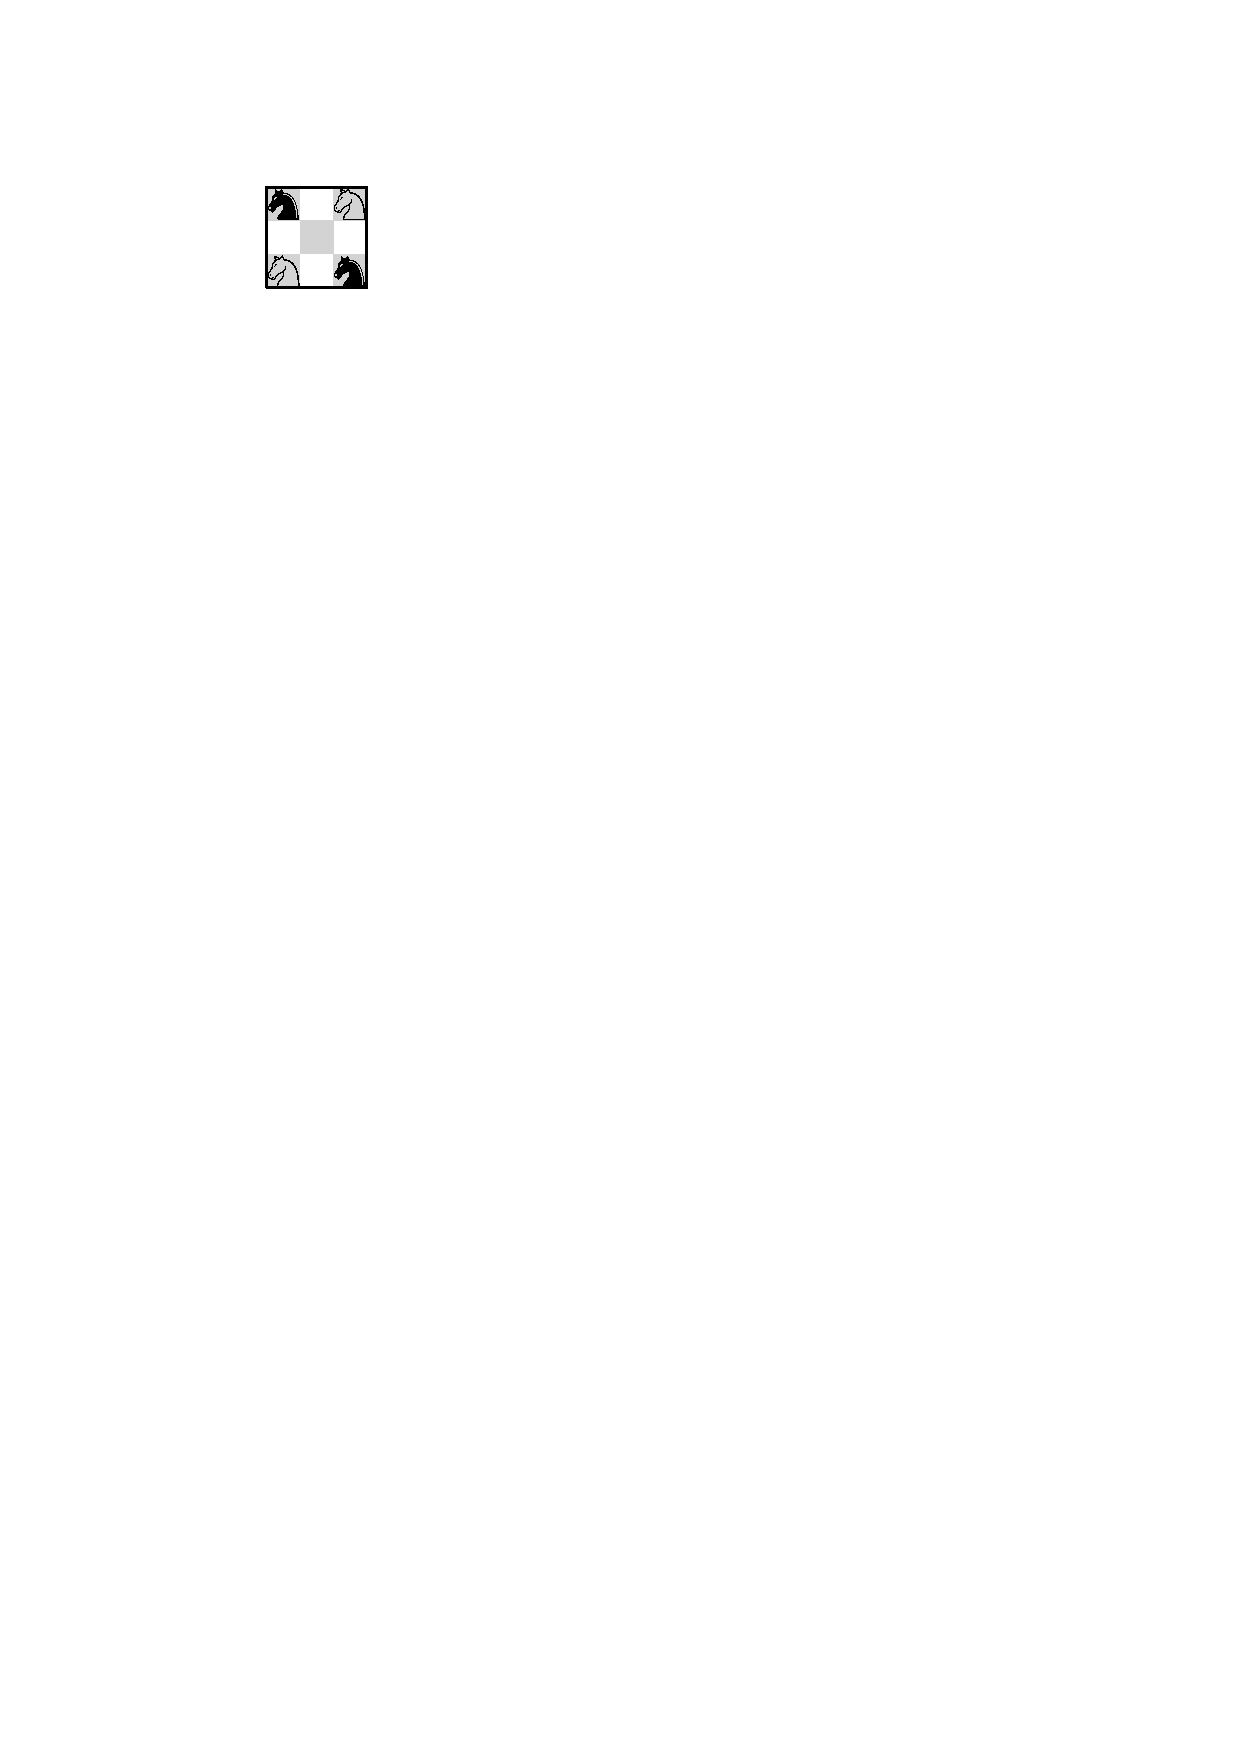
\includegraphics[scale=1.5]{img/Knights2.pdf}
\end{center}
\textbf{Решение:} \\

\begin{center}
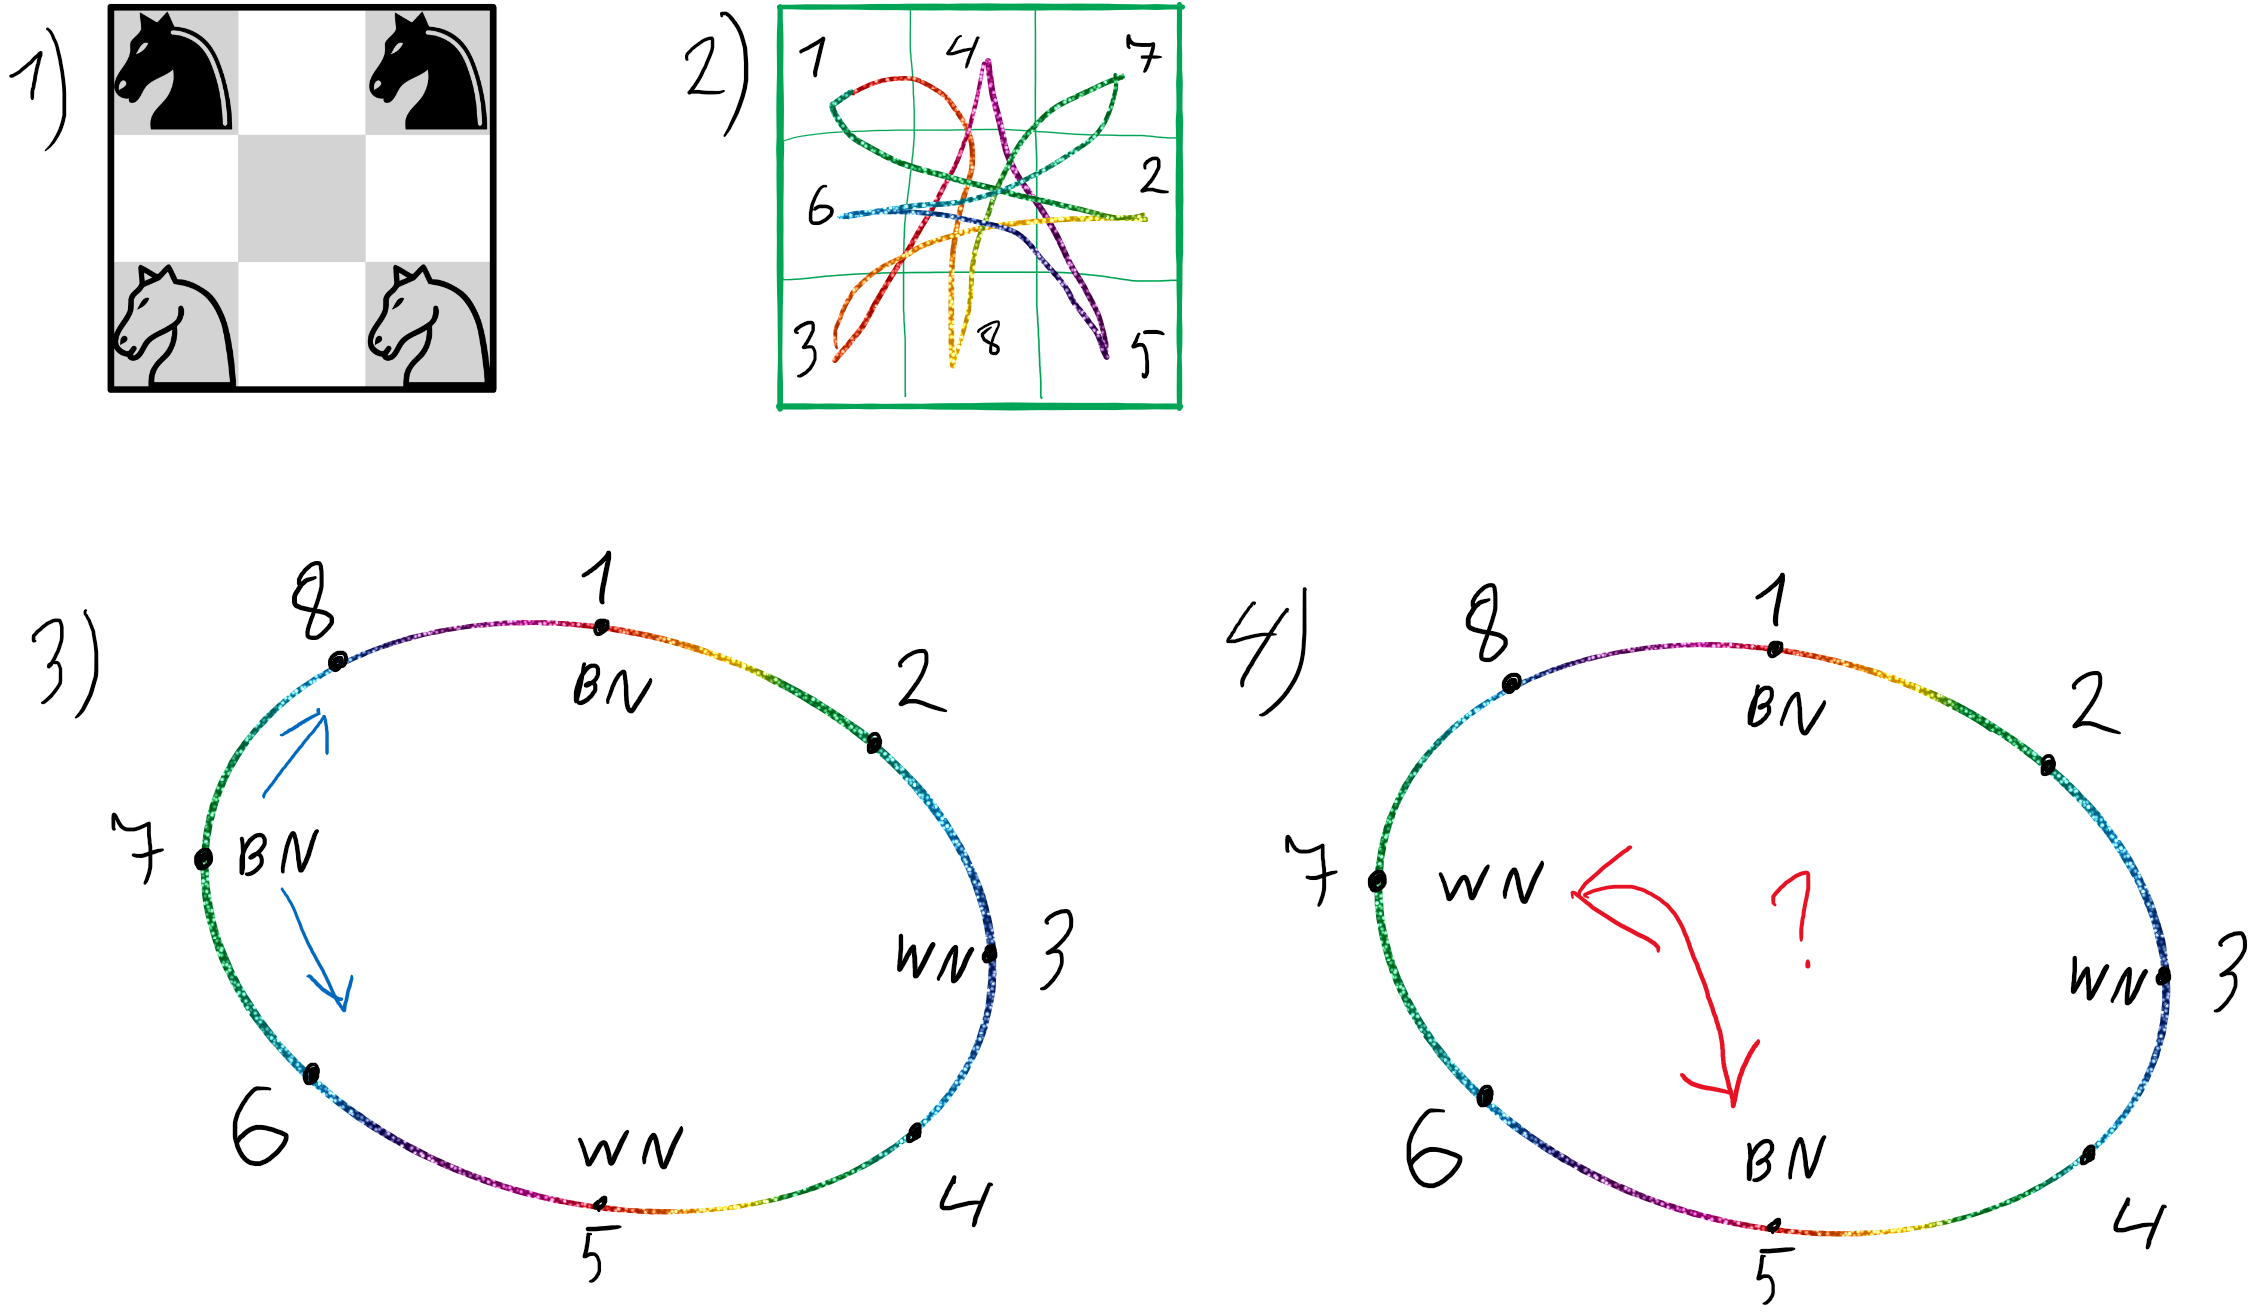
\includegraphics[width=\textwidth]{img/knights.png}
\end{center}

Еще раз посмотрим на исходное положение коней 1). Предположим, что у нас есть только один конь в верхнем левом углу доски.
На 2) нарисуем все возможные положения, которые он может занять, ходя конем. Всего 8 позиций, после чего он приходит на исходную точку.

Нарисуем круговой маршрут, который может пройти черный конь из верхнего левого угла и отметим номера позиций на 3). Отметим на этом маршруте белых коней как WN, а черных как BN.

Заметим, что у каждого коня в исходном положении - только 2 возможных хода (например из 7 позиции в 8 или 6).

Нарисуем на круговом маршруте финальное положение коней, которое спрашивается в задании. Это график 4). Он отличается от исходного 3) тем, что конь в положении 7 и 5 поменяны местами.

Так как кони перемещаясь из конфигурации 3) по круговому маршруту не могут занимать вдвоем 1 положение и не могут перемещаться только на 1 соседнюю позицию, для них всегда будет сохранятся соотношение:

а) Для каждого BN спереди и сзади по ходу движения есть 1 BN и 1 WN

б) Для каждого WN спереди и сзади по ходу движения есть 1 BN и 1 WN

При этом а) и б) будут верны как бы мы не перемещали коней.

В требуемой позиции:

в) для каждого WN - спереди и сзади есть 2 BN 

г) для каждого BN - спереди и сзади есть 2 WN.

в) и г) противоречат а) и б) $\Rightarrow$ нельзя перейти от одной позиции к другой


\textbf{Ответ: Нельзя, доказательство выше}

\end{document}